\chapter{Resultados}
\label{ch:resultados}

Este capítulo presenta la evaluación del modelo de extracción. Todas las medidas se han obtenido sobre el conjunto de validación, formado por 14 tickets reales (86 productos) que el modelo v3 no ha visto durante el entrenamiento.

\section{Métricas de evaluación}
Se han definido métricas a dos niveles, ticket y producto, alineadas con el objetivo planteado en la sección de objetivos (que la mayoría de los tickets se procesen de forma perfecta y que los fallos restantes sean menores):

\begin{itemize}
    \item \textbf{Ticket perfecto}: la fecha, el total y todos los productos (nombre, cantidad, precio unitario, peso e importe) coinciden exactamente con el \textit{Ground Truth}.
    \item \textbf{Ticket casi perfecto}: la fecha y el total son correctos y, como mucho, dos productos presentan algún fallo.
    \item \textbf{F1 de productos}: media armónica de la precisión ($P$, proporción de productos predichos que son correctos) y la exhaustividad ($R$, proporción de productos reales que se han predicho correctamente), $F_1 = 2PR/(P+R)$. Un producto se considera correcto si coinciden su nombre, su cantidad y su importe.
    \item \textbf{Acierto del total} y \textbf{acierto de la fecha}.
\end{itemize}

\section{Evolución durante el entrenamiento}
El entrenamiento se detuvo tras la sexta época por el criterio de parada temprana, con una duración total de 3 horas y 23 minutos (1.548 pasos de optimización). La tabla~\ref{tab:evolucion} recoge las métricas de validación al final de cada época y la figura~\ref{fig:curvas} muestra la evolución de la función de pérdida.

\begin{table}[htbp]
    \caption{\label{tab:evolucion}Métricas de validación del modelo v3 por época}
    \begin{tabularx}{\textwidth}{@{}cXXXX@{}}
        \toprule
        \textbf{Época} & \textbf{Pérdida (val.)} & \textbf{Tickets perfectos} & \textbf{Casi perfectos} & \textbf{F1 productos} \\
        \midrule
        1 & 0,0140 & 78,6\,\% & 100\,\% & 96,5\,\% \\
        2 & 0,0089 & 92,9\,\% & 100\,\% & 98,8\,\% \\
        3 & 0,0044 & 100\,\% & 100\,\% & 100\,\% \\
        4 & 0,0067 & 100\,\% & 100\,\% & 100\,\% \\
        5 & 0,0051 & 100\,\% & 100\,\% & 100\,\% \\
        6 & 0,0042 & 100\,\% & 100\,\% & 100\,\% \\
        \bottomrule
    \end{tabularx}
\end{table}

\begin{figure}[htbp]
    \centering
    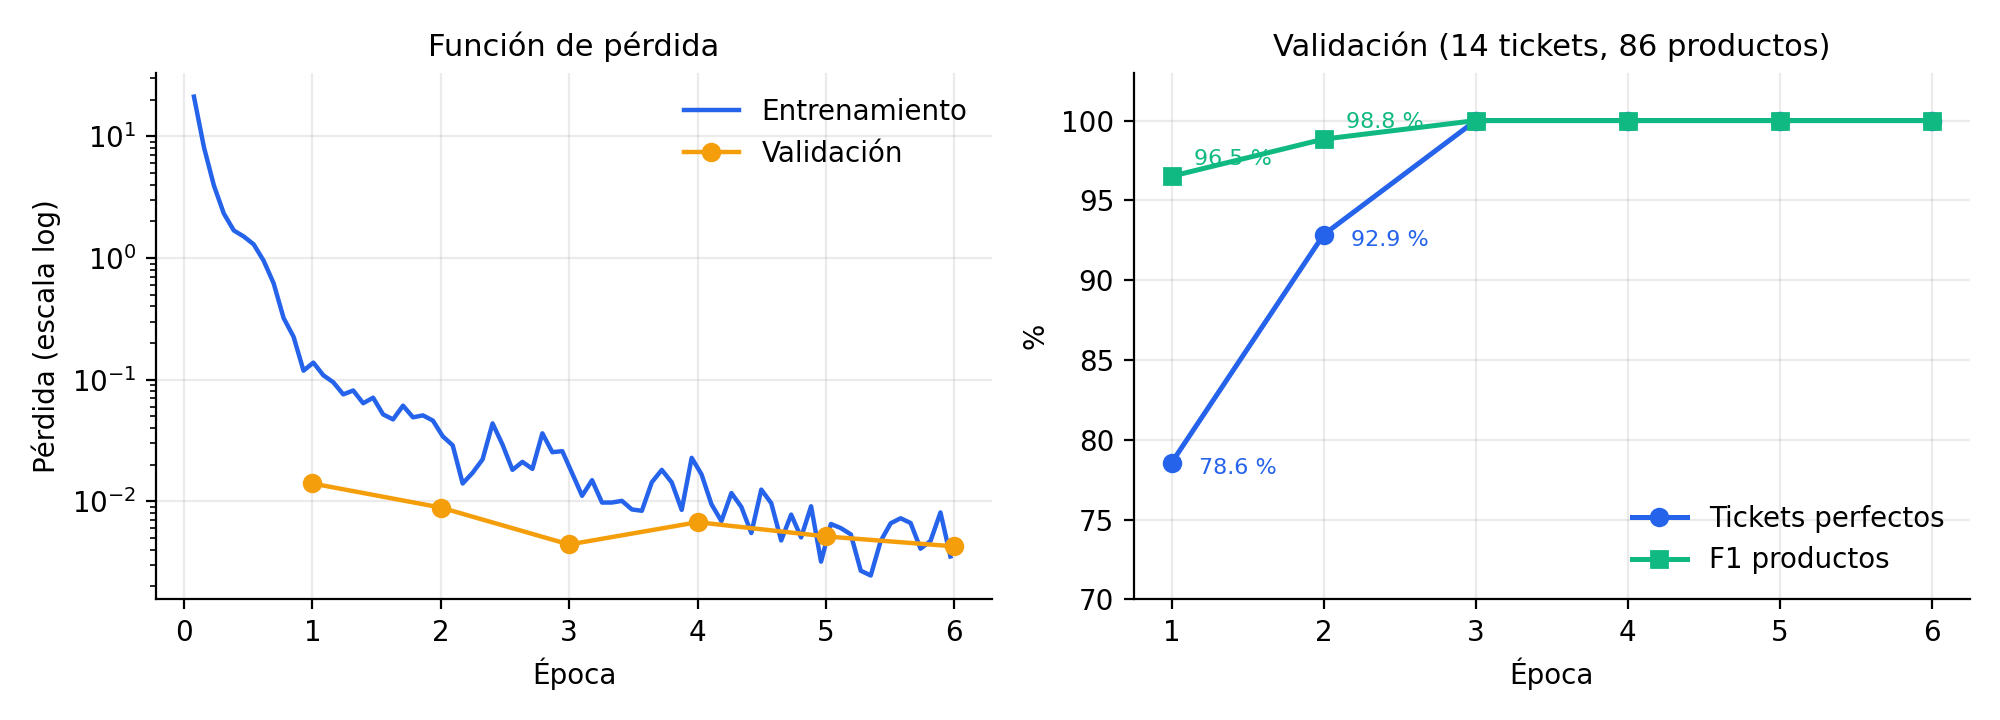
\includegraphics[width=\textwidth]{figuras/curva_entrenamiento.png}
    \caption{Pérdida de entrenamiento y validación (izquierda, escala logarítmica) y métricas de validación por época (derecha).}
    \label{fig:curvas}
\end{figure}

Ya desde la primera época ningún ticket presenta más de dos fallos y el total y la fecha se aciertan siempre. A partir de la tercera época el modelo lee correctamente los 14 tickets de validación. La pérdida de validación desciende junto con la de entrenamiento y no muestra una tendencia creciente, lo que indica que no se produce sobreajuste apreciable en el número de épocas empleado.

\section{Resultado final}
El modelo seleccionado obtiene sobre el conjunto de validación:

\begin{itemize}
    \item 14 de 14 tickets perfectos (100\,\%) y 86 de 86 productos correctos (F1 = 100\,\%).
    \item 100\,\% de acierto en el total y en la fecha.
    \item Un tiempo de inferencia de unos 2,4 segundos por ticket en la GPU T4.
\end{itemize}

El objetivo establecido al inicio del proyecto, que entre un 50 y un 60\,\% de los tickets se procesaran de forma perfecta, queda ampliamente superado.

\section{Comparación con la primera versión}
\label{s:comparacion}
Para cuantificar el efecto de los cambios descritos en la sección~\ref{s:diagnostico}, se ha evaluado el sistema de la primera iteración (modelo v2 junto con su post-procesado) sobre los mismos 14 tickets y con las mismas métricas. Hay que tener en cuenta que el modelo v2 se entrenó con los 91 tickets, por lo que ya había visto los tickets de validación y su resultado es optimista.

% TODO: completar con los resultados del cuaderno Comparacion_v2_v3.ipynb
% (la celda final imprime esta tabla directamente en LaTeX)
\begin{table}[htbp]
    \caption{\label{tab:comparacion}Comparación del sistema v2 y v3 sobre el conjunto de validación}
    \begin{tabularx}{\textwidth}{@{}Xrr@{}}
        \toprule
        \textbf{Métrica} & \textbf{v2} & \textbf{v3} \\
        \midrule
        Tickets perfectos (\%) & -- & 100,0 \\
        Tickets casi perfectos (\%) & -- & 100,0 \\
        F1 de productos (\%) & -- & 100,0 \\
        F1 solo de nombres de producto (\%) & -- & 100,0 \\
        Acierto del total (\%) & -- & 100,0 \\
        Acierto de la fecha (\%) & -- & 100,0 \\
        Salida estructurada válida (\%) & -- & 100,0 \\
        \bottomrule
    \end{tabularx}
\end{table}

\section{Discusión}
\subsection{Generalización}
Un resultado del 100\,\% obliga a comprobar que el modelo no se limita a memorizar. Dos evidencias indican que realmente lee el documento:

\begin{itemize}
    \item 31 de los 86 productos de validación (36\,\%) tienen nombres que no aparecen en ningún ticket real de entrenamiento, y todos se leen correctamente.
    \item Solo uno de los 14 tickets de validación contiene exactamente la misma lista de productos que algún ticket de entrenamiento.
\end{itemize}

\subsection{Incertidumbre de la medida}
El conjunto de validación es pequeño. Con 14 aciertos sobre 14 tickets, el intervalo de confianza al 95\,\% de Clopper-Pearson para la proporción de tickets perfectos es $[76{,}8\,\%,\;100\,\%]$. Por tanto, el resultado debe interpretarse como que el sistema procesa de forma perfecta, con alta probabilidad, más de tres de cada cuatro tickets de este tipo, y no como una garantía de acierto total.

\subsection{Factores determinantes}
La comparación entre ambas iteraciones muestra que la mejora no procede de cambiar de modelo, ya que ambas versiones parten del mismo Donut preentrenado, sino principalmente de la corrección del conjunto de datos y de la adaptación del modelo al problema: etiquetas validadas, un formato de salida adecuado, una resolución suficiente y la ampliación del vocabulario. Este resultado está en línea con el enfoque centrado en los datos (\textit{data-centric AI}), según el cual mejorar la calidad de los datos suele aportar más que ajustar el modelo.

\subsection{Limitaciones}
\begin{itemize}
    \item El modelo solo se ha evaluado con tickets digitales de Mercadona, que comparten una maqueta fija. No se ha comprobado su comportamiento con fotografías de tickets impresos (iluminación, perspectiva, papel térmico) ni con otras cadenas de supermercados.
    \item El conjunto de validación (14 tickets) limita la precisión de la estimación.
    \item La categorización automática depende del catálogo de Mercadona: un 4\,\% de los nombres de producto no encuentra correspondencia y debe asignarse manualmente.
\end{itemize}
